\documentclass{scrartcl}

\usepackage[left=0.5cm, right=1cm, top=1.5cm]{geometry}		%decrease margins
\usepackage{tikz}

%color signal waveforms 
%from Middleton, R. (1969). Using Scopes in Color TV. Carmel, IN: Howard W. Sams & Co.
%image via https://thediagram.com/9_3/colorsignal.html

\begin{document}
	
	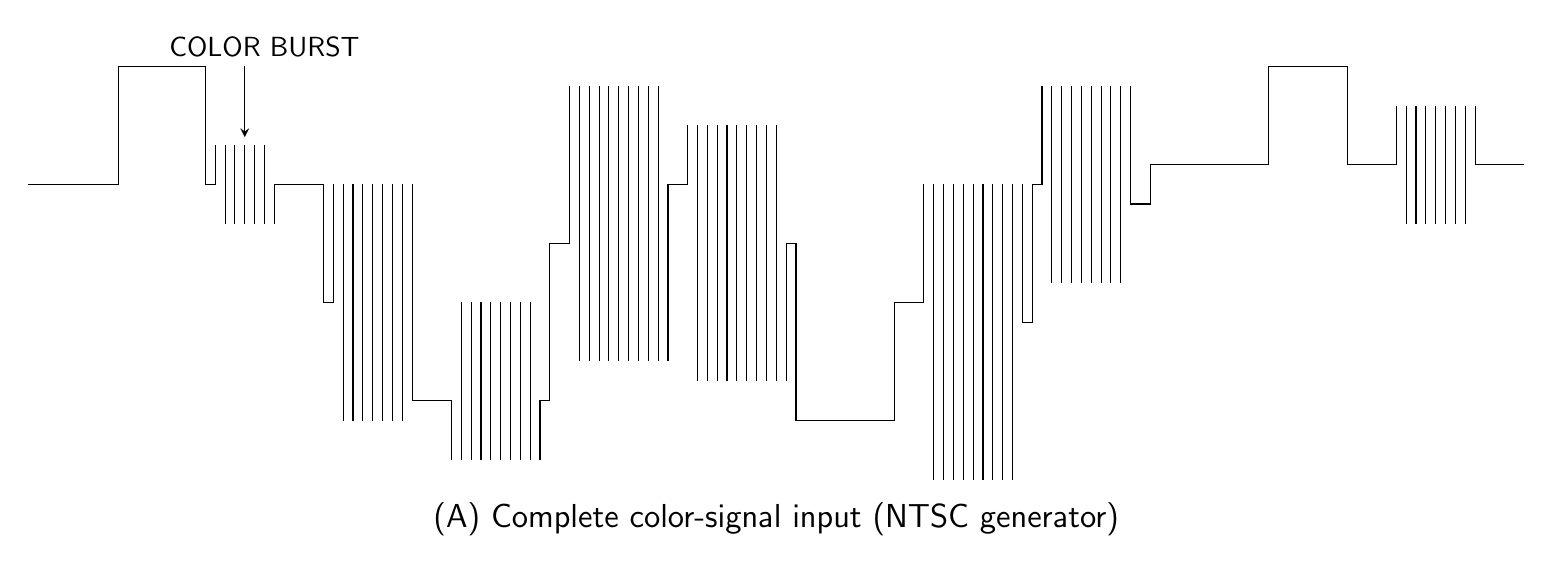
\begin{tikzpicture}
	\draw (-2.5,0)--(-1.35,0)--(-1.35,1.5)--(-0.25,1.5)--(-0.25,0)--(-0.125,0)--(-0.125,0.5); %handle
	
	%ONE
	\foreach \x in {0,...,4}
	\draw (\x*0.125,0.5)--(\x*0.125,-0.5);
	
	\draw (0.625,-0.5)--(0.625,0)--(1.25,0)--(1.25,-1.5)--(1.375,-1.5)--(1.375,0);
	
	%TWO
	\foreach \x in {0,...,6}
	\draw (1.5+\x*0.125,0)--(1.5+\x*0.125,-3);
	
	\draw (2.375,0)--(2.375,-2.75)--(2.875,-2.75)--(2.875,-3.5);
	
	%THREE
	\foreach \x in {0,...,7}
	\draw (3+\x*0.125,-1.5)--(3+\x*0.125,-3.5);
	
	\draw (4,-3.5)--(4,-2.75)--(4.125,-2.75)--(4.125,-0.75)--(4.375,-0.75)--(4.375,1.25);
	
	%FOUR
	\foreach \x in {0,...,8}
	\draw (4.5+\x*0.125,1.25)--(4.5+\x*0.125,-2.25);
	
	\draw (5.625,-2.25)--(5.625,0)--(5.875,0)--(5.875,0.75);
	
	%FIVE
	\foreach \x in {0,...,8}
	\draw (6+\x*0.125,0.75)--(6+\x*0.125,-2.5);
	
	\draw (7.125,-2.5)--(7.125,-0.75)--(7.25,-0.75)--(7.25,-3)--(8.5,-3)--(8.5,-1.5)--(8.875,-1.5)--(8.875,0);
	
	%SIX
	\foreach \x in {0,...,8}
	\draw (9+\x*0.125,0)--(9+\x*0.125,-3.75);
	
	\draw (10.125,0)--(10.125,-1.75)--(10.25,-1.75)--(10.25,0)--(10.375,0)--(10.375,1.25);
	
	%SEVEN
	\foreach \x in {0,...,7}
	\draw (10.5+\x*0.125,1.25)--(10.5+\x*0.125,-1.25);
	
	\draw (11.5,1.25)--(11.5,-0.25)--(11.75,-0.25)--(11.75,0.25) -- (13.25,0.25)--(13.25,1.5)--(14.25,1.5)--(14.25,0.25)--(14.875,0.25)--(14.875,1);
	
	%EIGHT
	\foreach \x in {0,...,6}
	\draw (15+\x*0.125,1)--(15+\x*0.125,-0.5);
	
	\draw (15.875,1)--(15.875,0.25)--(16.5,0.25);
	
	%LABELS
	\draw[->,>=stealth] (0.25,1.5)--(0.25,0.6);
	\node at (0.5,1.75) {\textsf{COLOR BURST}};
	\node at (7,-4.25) {\large \textsf{(A) Complete color-signal input (NTSC generator)}};
	
	%\draw[help lines] (-2,-2) grid (16,2);	\fill[red] (0,0) circle (2pt);
	\end{tikzpicture}
	
	
	\vspace{0.35cm}
	
	
	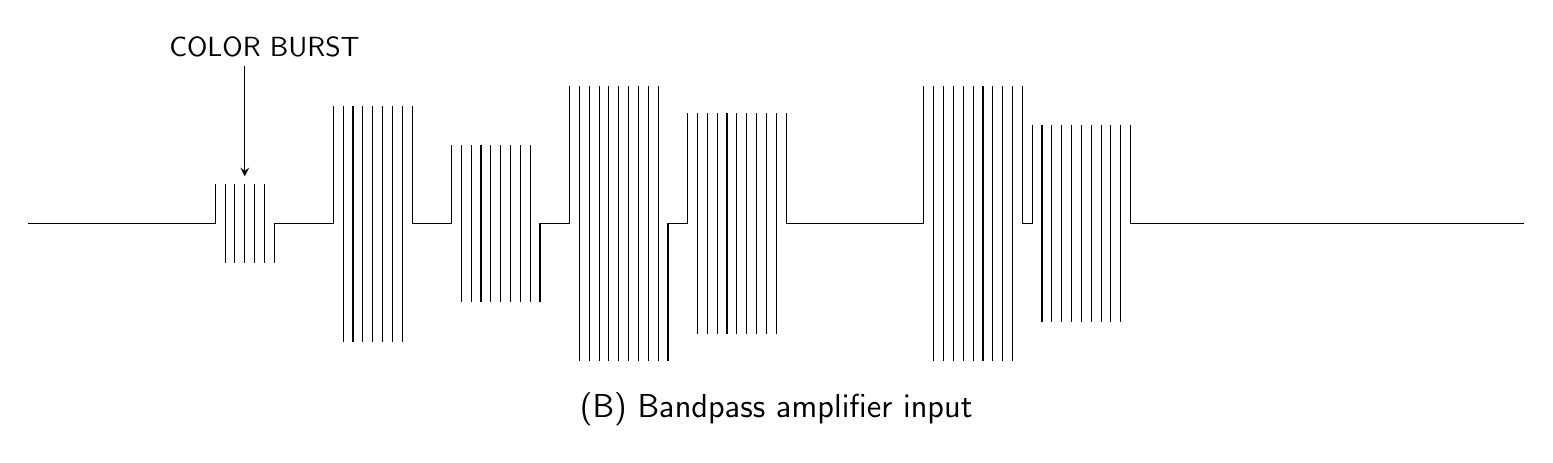
\begin{tikzpicture}
	\draw (-2.5,0)--(-0.125,0)--(-0.125,0.5);	%leftward handle
	
	%ONE
	\foreach \x in {0,...,4}
	\draw (\x*0.125,0.5)--(\x*0.125,-0.5);
	
	\draw (0.625,-0.5)--(0.625,0)--(1.375,0)--(1.375,1.5);
	
	%TWO
	\foreach \x in {0,...,6}
	\draw (1.5+\x*0.125,1.5)--(1.5+\x*0.125,-1.5);
	
	\draw (2.375,1.5)--(2.375,0)--(2.875,0)--(2.875,1);
	
	%THREE
	\foreach \x in {0,...,7}
	\draw (3+\x*0.125,1)--(3+\x*0.125,-1);
	
	\draw (4,-1)--(4,0)--(4.375,0)--(4.375,1.75);
	
	%FOUR
	\foreach \x in {0,...,8}
	\draw (4.5+\x*0.125,1.75)--(4.5+\x*0.125,-1.75);
	
	\draw (5.625,-1.75)--(5.625,0)--(5.875,0)--(5.875,1.4);
	
	%FIVE
	\foreach \x in {0,...,8}
	\draw (6+\x*0.125,1.4)--(6+\x*0.125,-1.4);
	
	\draw (7.125,1.4)--(7.125,0)--(8.875,0)--(8.875,1.75);
	
	%SIX
	\foreach \x in {0,...,8}
	\draw (9+\x*0.125,1.75)--(9+\x*0.125,-1.75);
	
	\draw (10.125,1.75)--(10.125,0)--(10.25,0)--(10.25,1.25);
	
	%SEVEN
	\foreach \x in {0,...,8}
	\draw (10.375+\x*0.125,1.25)--(10.375+\x*0.125,-1.25);
	
	\draw (11.5,1.25)--(11.5,0)--(16.5,0);
	
	%LABELS
	\draw[->,>=stealth] (0.25,2)--(0.25,0.6);
	\node at (0.5,2.25) {\textsf{COLOR BURST}};
	\node at (7,-2.35) {\large \textsf{(B) Bandpass amplifier input}};
	%\draw[help lines] (-2,-2) grid (16,2);	\fill[red] (0,0) circle (2pt);
	\end{tikzpicture}
	
	
	\vspace{0.35cm}
	
	
	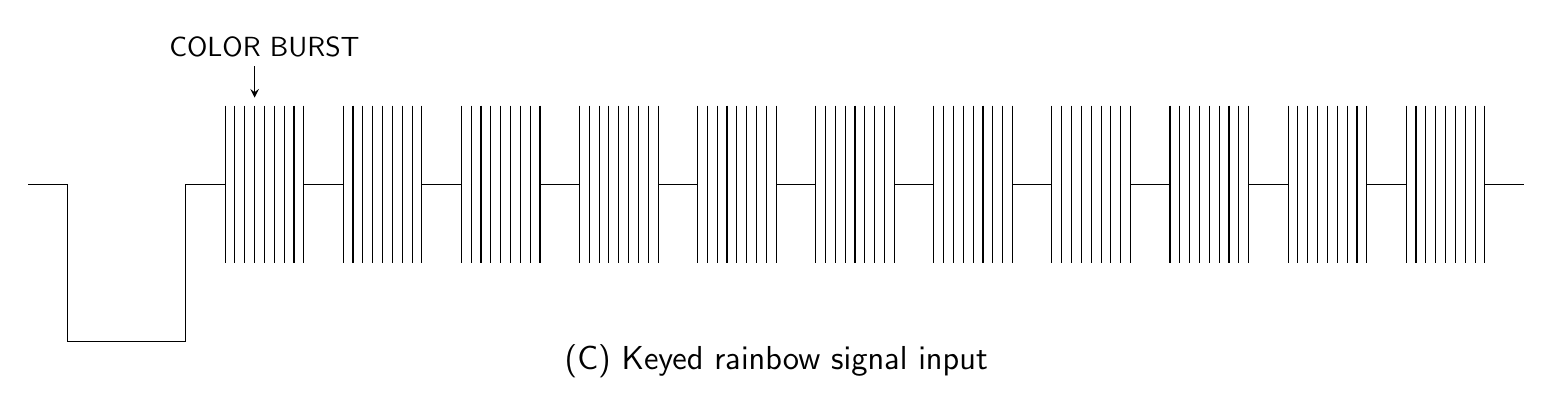
\begin{tikzpicture}
	\draw (-2.5,0)--(-2,0)--(-2,-2)--(-0.5,-2)--(-0.5,0)--(0,0);	%leftward handle

	\foreach \n in {0,...,10}{
	\foreach \x in {0,...,8} 
	\draw (1.5*\n + \x*0.125,1)--(1.5*\n + \x*0.125,-1);
	\draw (1+1.5*\n,0)--(1.5+1.5*\n,0);
	}

	%LABELS
	\draw[->,>=stealth] (0.375,1.5)--(0.375,1.1);
	\node at (0.5,1.75) {\textsf{COLOR BURST}};
	\node at (7,-2.25) {\large \textsf{(C) Keyed rainbow signal input}};
	%\draw[help lines,red] (0,-1) grid (16,1);
	\end{tikzpicture}
	
	
	\vspace{0.5cm}
	
	
	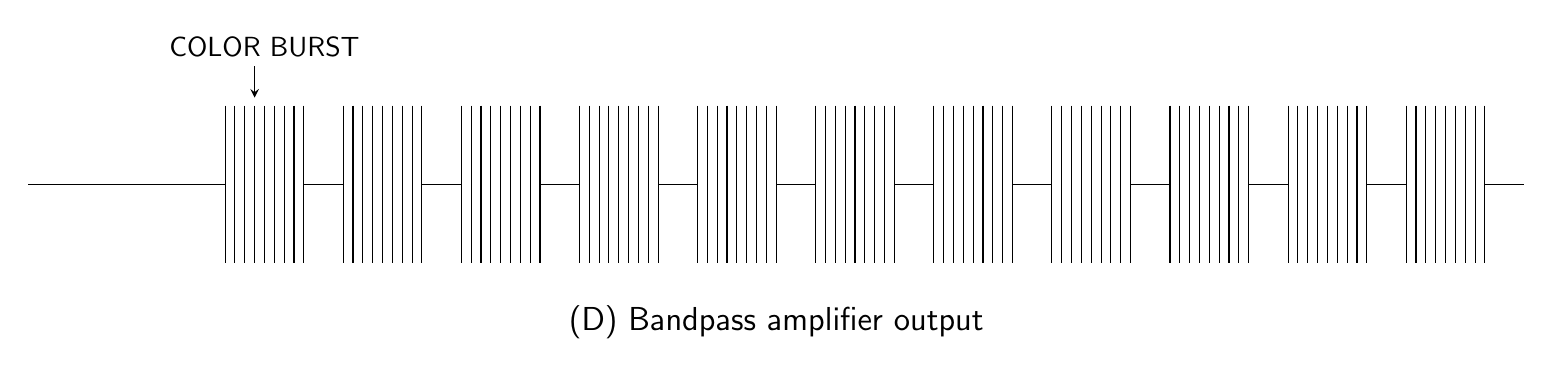
\begin{tikzpicture}
	\draw (-2.5,0)--(0,0);		%leftward handle
	\foreach \n in {0,...,10}{
		\foreach \x in {0,...,8} 
		\draw (1.5*\n + \x*0.125,1)--(1.5*\n + \x*0.125,-1);
		\draw (1+1.5*\n,0)--(1.5+1.5*\n,0);
	}
	%LABELS
	\draw[->,>=stealth] (0.375,1.5)--(0.375,1.1);
	\node at (0.5,1.75) {\textsf{COLOR BURST}};
	\node at (7,-1.75) {\large \textsf{(D) Bandpass amplifier output}};
	\end{tikzpicture}
	
	
\end{document}